% Copyright (C) 2014-2020 by Thomas Auzinger <thomas@auzinger.name>

\documentclass[draft,final]{vutinfth} % Remove option 'final' to obtain debug information.

% Load packages to allow in- and output of non-ASCII characters.
\usepackage{lmodern}        % Use an extension of the original Computer Modern font to minimize the use of bitmapped letters.
\usepackage[T1]{fontenc}    % Determines font encoding of the output. Font packages have to be included before this line.
\usepackage[utf8]{inputenc} % Determines encoding of the input. All input files have to use UTF8 encoding.

% Extended LaTeX functionality is enables by including packages with \usepackage{...}.
\usepackage{amsmath}    % Extended typesetting of mathematical expression.
\usepackage{amssymb}    % Provides a multitude of mathematical symbols.
\usepackage{mathtools}  % Further extensions of mathematical typesetting.
\usepackage{microtype}  % Small-scale typographic enhancements.
\usepackage[inline]{enumitem} % User control over the layout of lists (itemize, enumerate, description).
\usepackage{multirow}   % Allows table elements to span several rows.
\usepackage{booktabs}   % Improves the typesettings of tables.
\usepackage{subcaption} % Allows the use of subfigures and enables their referencing.
\usepackage[ruled,linesnumbered,algochapter]{algorithm2e} % Enables the writing of pseudo code.
\usepackage[usenames,dvipsnames,table]{xcolor} % Allows the definition and use of colors. This package has to be included before tikz.
\usepackage{nag}       % Issues warnings when best practices in writing LaTeX documents are violated.
\usepackage{todonotes} % Provides tooltip-like todo notes.
\usepackage{hyperref}  % Enables cross-linking in the electronic document version. This package has to be included second to last.
\usepackage[acronym,toc]{glossaries} % Enables the generation of glossaries and lists fo acronyms. This package has to be included last.
\usepackage{float}
\usepackage{amsfonts,amsthm, graphicx, trfsigns, physics, xparse, mleftright, listings, xurl}

\begin{document}

    \title{\textbf{Master Thesis Proposal}\\Neural Network Arena: Comparing Machine Learning Models using Long-Term Dependency and Physical System Time Series Benchmarks}
    \author{Faculty Supervisor: Univ.-Prof. Dipl.-Ing. Dr.rer.nat. Radu Grosu\\ Direct Supervisor: Dr. Ramin Hasani \\ Student: Hannes Brantner (01614466)}
    \maketitle{}

% Select the language of the thesis, e.g., english or naustrian.
    \selectlanguage{english}


    \chapter{Proposal}


    \section{Machine Learning Terms}
    A machine learning model is a mathematical parametrized function that gets input and produces an output.
    For example, the machine learning model GPT-3 proposed in \cite{GPT-3} has 175 billion scalar parameters.
    This thesis will use imitation learning to set the parameters of machine learning models optimally.
    Imitation learning means an associative expected output provided for each input that the model should return by applying its function to the input.
    Of course, when the model's function is applied to the input with the model's parameters' initial state, the returned model output will differ from the desired output in almost all cases.
    The measure responsible for quantifying this error between model output and the expected output is called a loss function and has a scalar return value.
    A sample loss function can be constructed quickly by computing the mean of all squared errors between the model output and the expected output.
    The model output is also often denoted as the prediction of the model.
    For each input sample, the loss function describes the error the model makes by applying its function, and this error is only dependent on the model's parameters.
    In practice, the loss function is applied to a batch of inputs separately, and the arithmetic mean of all scalar loss function return values of the individual input samples is used as a loss function to differentiate.
    The size of this input batch is called batch size.
    A computer scientist wants to find the global minimum of that function concerning all machine learning model parameters in the general case.
    A visualized loss surface where the loss function return value is plotted in the z-axis and all possible model parameter combinations are given as points on the plane is given as follows:
    \begin{figure}[H]
        \centering{}
        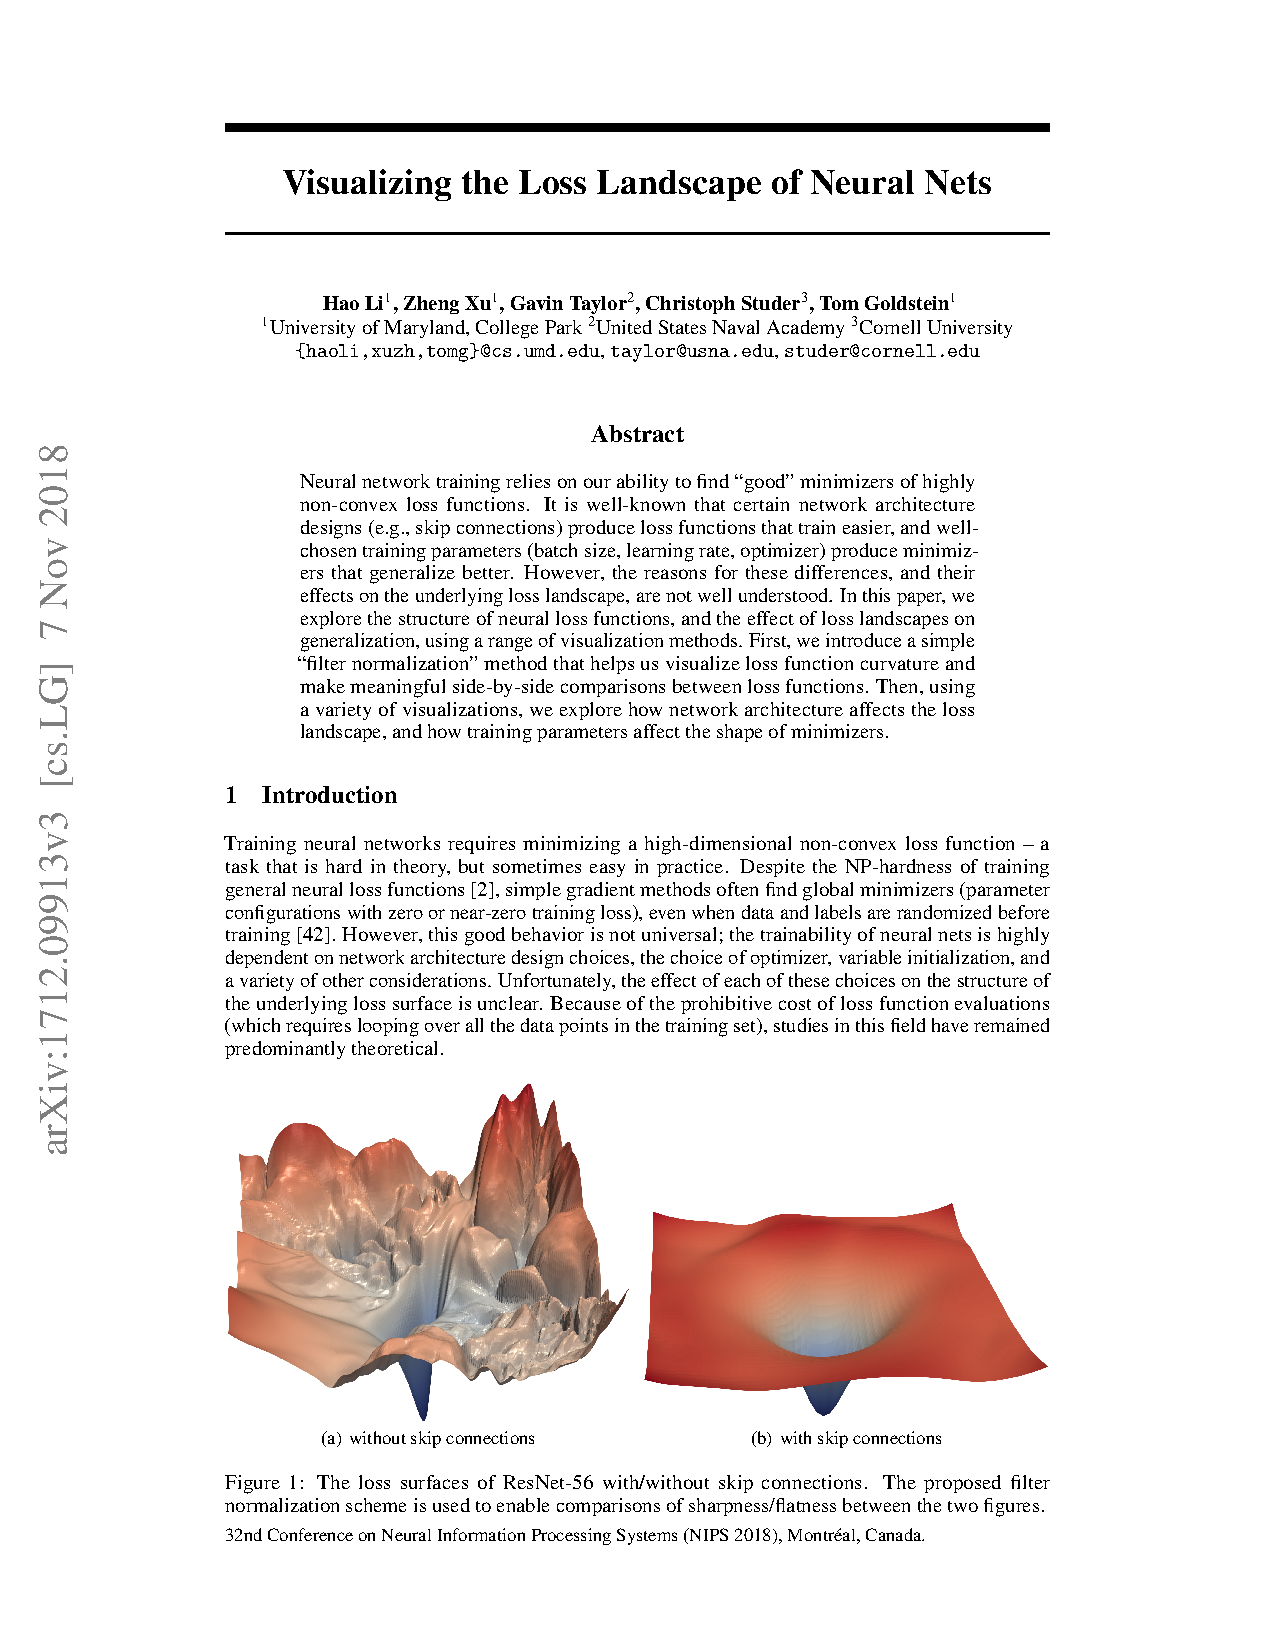
\includegraphics[page=1,width=0.8\linewidth,trim={105 107 305 510},clip]{literature/visualizing_the_loss_landscape_of_neural_nets.pdf}
        \caption{visualized loss surface \cite[p. 1]{loss_vis}}
        \label{fig:loss_vis}
    \end{figure}
    As this is a problem that cannot be solved analytically in most cases, it is approximated by using gradient descent \cite{GradientDescent}.
    This method incrementally changes each parameter depending on the gradient of each parameter's loss function in a lockstep fashion.
    By denoting the loss function with $L$, the learning rate with $\alpha$, the whole old parameter set with $p$, the old single scalar parameter with $p_i$ and the new single scalar parameter with $p_i'$, the formula to update the individual parameters $p_i$ in a single gradient descent step can be given as follows \cite{GradientDescent}:
    \begin{align}
        \label{gradient_descent_update}
        \forall p_i:~p_i' &= p_i - \alpha * \frac{\partial{L}}{\partial{p_i}}(p)
    \end{align}
    It is essential to note that the model and the loss measure must be deterministic functions for the gradient to exist.
    This update rule ensures that if the loss function increases with increasing $p_i$, a decrease of the parameter will happen, leading to a decreasing loss function result.
    The opposite case holds as well, and this is why there is a minus sign in \ref{gradient_descent_update}.
    The learning rate $\alpha$ determines how significant in magnitude the update to the parameters should be at each gradient descent step.
    A too-small learning rate will lead to slow convergence, and a too-large learning rate will lead to divergence.
    Therefore, a too-large learning rate is far more dangerous than a too-small one.
    Convergence means that the parameter updates have led to a local minimum of the loss function.
    There are no guarantees that this is the global minimum. Divergence means that the loss function diverges towards infinity.
    A local minimum or convergence can be reached by applying the gradient descent update rule to as many inputs as needed to set the loss function derivative to nearly zero.
    The trajectory of the parameter set on the loss surface when repeatedly applying the gradient descent update rule was visualized in \cite[p. 2]{gradient_descent_vis} with the initial starting parameter set denoted as a black triangle as follows:
    \begin{figure}[H]
        \centering{}
        \includegraphics[page=2,width=0.8\linewidth,trim={90 585 355 75},clip]{literature/gradvis_visualization_and_second_order_analysis_of_optimization_surfaces_during_the_training_of_deep_neural_networks.pdf}
        \caption{visualization of gradient descent}
        \label{fig:gradient_descent_vis}
    \end{figure}
    The differentiation of the loss function, which can be represented as a computational graph with lots of nested functions, involves many chain rule applications for the individual model parameter derivatives. The machine learning term for repeatedly applying the chain rule is backpropagation.
    If these nested functions correspond to applying the same machine learning model function across multiple input time steps as done in recurrent neural networks, then this backpropagation procedure can also be called backpropagation through time as introduced in \cite{GradientDescent}.
    The chain rule for differentiating $z(y(x_0))$ with respect to $x$ for $x=x_0$ where $z$ and $y$ are both functions in a single variable is given by:
    \begin{align}
        \label{chain_rule}
        \frac{dz}{dx} \Bigr\rvert_{x=x_0} = \frac{dz}{dy} \Bigr\rvert_{y=y(x_0)} * \frac{dy}{dx} \Bigr\rvert_{x=x_0}
    \end{align}
    The above equation reveals that a machine learning framework has to compute all partial derivatives of all functions present in the above-mentioned computational graph.
    Furthermore, it must keep track of the so-called activations, which are denoted by $y(x_0)$ in the above formula \ref{chain_rule}, as otherwise the gradient of the loss function with respect to the individual parameters cannot be computed.
    As this can use lots of memory, reversible layers were introduced by \cite{ReversibleLayer} where intermediate activations can be computed from the layer's output vector, which makes storing intermediate activations obsolete.


    \section{Problem Statement}
    As the sheer amount of different machine learning models can be overwhelming, the task was to fix a distinct application domain and compare the most influential machine learning models in this domain with suitable benchmarks.
    Benchmarks are just large input data sets with associative expected outputs.
    Additionally, ideas for possible improvements in existing architectures should be implemented and benchmarked against existing ones.
    All benchmarked models should be implemented in the same machine learning framework, and the benchmark suite should be extensible and reusable for other machine learning research projects.
    The whole implementation work done for this thesis should be accessible for everyone by open-sourcing all the code.
    As mentioned in the abstract, all the models covered in this thesis are either derivatives of the recurrent neural network or the transformer \cite{Transformer} architecture.
    The benchmarks used in this thesis either test the models for their capabilities to capture long-term dependencies or their ability to model physical systems.


    \section{How to better model Physical Systems} \label{physical_systems}
    Differential equations guide physical systems. The relation between system state $x$, system input $u$ and system output $y$ is given by the state derivative function $f$ and the output function $h$, both of which depend on the absolute time $t$, as follows:
    \begin{align}
        \label{physical_system_equations_state}
        \dot x(t) &= f(x(t),u(t),t) \\
        \label{physical_system_equations_output}
        y(t) &= h(x(t),u(t),t)
    \end{align}
    This form of system description applies to all continuous physical systems in our daily surroundings. Most of these systems are even time-invariant.
    This means the functions $f$ and $h$ do not depend on the absolute time $t$.
    For example, a mechanical pendulum will now approximately behave the same as in one year, as its dynamics do not depend on the absolute time $t$.
    The system description presented in \ref{physical_system_equations_state} and \ref{physical_system_equations_output} proposes that machine learning models built similarly and whose state is also determined by a differential equation should be pretty capable of modeling the input-output relation of physical systems.
    When the benchmarked models are introduced in more detail, it can be seen that all continuous-time machine learning models use a comparable structure in terms of parameterizing the state derivative and the output function.
    The key takeaway point is that continuous physical systems map an input function $x(t)$ to an output function $y(t)$ as visualized in \cite[p. 102]{dsp}:
    \begin{figure}[H]
        \centering{}
        \includegraphics[page=102,width=0.8\linewidth,trim={110 580 140 60},clip]{literature/digital_signal_processing.pdf}
        \caption{visualization of input-output relation of a continuous system}
        \label{fig:continuous_system_vis}
    \end{figure}


    \section{Sampled Physical Systems} \label{sampled_physical_systems}
    As the current state's evaluation $x$ at time point $t'$, with initial state $x_0$ given the dynamics from \ref{physical_systems}, can be computationally very expensive or even infeasible, sampling was introduced to avoid solving a complex differential equation.
    Therefore, the whole system is only observed at equidistant successive time instants, values belonging to this time instant are denoted with a subscript index $k \in \mathbb{Z}$, and the system is now called discrete.
    Difference equations guide discrete systems. The relation between system state $x$, system input $u$ and system output $y$ is given by the next state function $f$ and the output function $h$, both of which depend on the time instant $k$, as follows:
    \begin{align}
        \label{discrete_system_equations_state}
        x_{k+1} &= f(x_k,u_k,k) \\
        \label{discrete_system_equations_output}
        y_k &= h(x_k,u_k,k)
    \end{align}
    It must be noted that $x$ and $y$ are time-series in discrete systems and no more functions like in continuous-time physical systems.
    This slightly off-topic explanation is necessary, as vanilla recurrent neural networks are built using the same principle.
    The system equations \ref{discrete_system_equations_state} and \ref{discrete_system_equations_output} require a regularly (equidistantly) sampled input $x$.
    A similar argument as before in \ref{physical_systems} proposes now that a machine learning model with a similar structure, which gets a regularly sampled input of a physical system, should also be pretty capable of modeling the input-output relation of this sampled physical system.
    The corresponding machine learning models are then called discrete-time machine learning models.
    The key takeaway point is that discrete physical systems map an input sequence $x[n]$ to an output sequence $y[t]$ as visualized in \cite[p. 102]{dsp}:
    \begin{figure}[H]
        \centering{}
        \includegraphics[page=102,width=0.8\linewidth,trim={110 485 140 150},clip]{literature/digital_signal_processing.pdf}
        \caption{visualization of input-output relation of a discrete system}
        \label{fig:discrete_system_vis}
    \end{figure}


    \section{Why capturing Long-Term Dependencies is difficult} \label{long_term_difficult}
    The difficulty will be outlined solely on the example of vanilla recurrent neural networks (RNNs).
    How transformer-based and advanced RNN architectures tackle the problem will be discussed later.
    Vanilla recurrent neural networks are discrete-time machine learning models.
    Its dynamics are given similar to the equations that govern sampled physical systems \ref{sampled_physical_systems}.
    The current state vector $h_{t}$ and the next input vector $x_{t+1}$ determine the next state vector $h_{t+1}$ and output vector $y_{t+1}$ deterministically.
    In this model, all the past inputs are implicitly encoded in the current state vector.
    This implicit encoding entails a big challenge for computer scientists, as computers only allow states of finite size and finite precision, unlike our physical environment, which results in an information bottleneck in the state vector.
    The next state of a vanilla recurrent neural network $h_{t+1}$ and its output $y_{t}$ is typically computed by equations like the two proposed in \cite[p. 2]{UnitaryRNNs} by using a non-linear bias-parametrized activation function $\sigma$, three matrices ($W$, $V$ and $U$) and the output bias vector $b_o$:
    \begin{align}
        \label{rnn_state_update}
        h_{t+1} &= \sigma(W*h_t + V*x_{t+1}) \\
        \label{rnn_output}
        y_{t} &= U*h_{t} + b_o
    \end{align}
    Without the time shift on the input in the next state equation \ref{rnn_state_update}, the equations are similar to those describing sampled physical systems.
    Equation \ref{rnn_state_update} can be visualized by the following figure:
    \begin{figure}[H]
        \centering{}
        \includegraphics[width=0.8\linewidth]{graphics/rnn.png}
        \caption{visualization of an RNN state update \cite{rnn_vis}}
        \label{fig:rnn_vis}
    \end{figure}
    The following inequality from \cite[p. 2]{UnitaryRNNs} using norms shows the relation between the loss derivative, a recent state $h_T$ and a state from the distant past $h_t$ where $T \gg t$.
    The notation is kept similar to the examples before. A subscript $2$ after a vector norm denotes the Euclidean norm, and a subscript $2,ind$ after a matrix norm denotes the spectral norm:
    \begin{align}
        \label{gradient_formula}
        \left\Vert \pdv{L}{h_t} \right\Vert_2 \leq \left\Vert \pdv{L}{h_T} \right\Vert_2 * \left\Vert W \right\Vert_{2,ind}^T * \prod^{T-1}_{k=t} \left\Vert diag(\sigma'(W*h_k + V*x_{k+1})) \right\Vert_{2,ind}
    \end{align}
    This inequality contains all essential parts to understand why capturing long-term dependencies with vanilla recurrent neural networks is difficult.
    Some problems that machine learning tries to solve require incorporating input data from the distant past to make good predictions in the present.
    As these inputs are implicitly encoded in the states of the distant past, $\left\Vert \pdv{L}{h_t} \right\Vert_2$ should not decay to zero or grow unboundedly to effectively tune the parameters using the gradient descent update rule shown above in \ref{gradient_descent_update}.
    This persistence of the gradient ensures that distant past inputs influence the loss function reasonably and makes it feasible to incorporate the knowledge to minimize the loss function.
    As known, the spectral norm of the diagonal matrix in \ref{gradient_formula} is just the largest magnitude out of all diagonal entries.
    Therefore, if the diagonal matrix's norm is close to zero over multiple time steps $k$, the desired loss gradient will decay towards zero.
    Otherwise, if the diagonal matrix's norm is much larger than one over multiple time steps $k$, the desired loss gradient may grow unboundedly.
    Using this knowledge, it is now clear that a suitable activation function must have a derivative of one in almost all cases to counteract the above-described problems.
    A good fit would be a rectified linear unit (relu) activation function with an added bias term.
    The relu activation function with a bias $b$ can simply be discribed by the function $max(0,x+b)$. The $max$ function should be applied element-wise.
    As the requirements for the activation function candidates are precisely formulated now, the next thing to discuss is the norm of the matrix $W$.
    If $\left\Vert W \right\Vert_{2,ind} > 1$, $\left\Vert \pdv{L}{h_t} \right\Vert$ may grow unboundedly, making it difficult to apply the gradient descent technique to optimize parameters.
    If $\left\Vert W \right\Vert_{2,ind} < 1$, $\left\Vert \pdv{L}{h_t} \right\Vert$ will decay to $0$, making it impossible to apply the gradient descent technique to optimize parameters.
    These problems are identical to the norm of the diagonal matrix and have the same implications.
    The first case is called the exploding gradient problem, and the second case is called the vanishing gradient problem for given reasons.
    Both phenomena are explained in more detail in \cite{LongTermDependenciesGradientDescent}.


    \section{Aim of the Work}
    This work should help to objectively compare various machine learning models used to process regularly sampled time-series data.
    It should outline the weaknesses and strengths of the benchmarked models and determine their primary domain of use.
    Moreover, as there are many models benchmarked, their relative expressivity across various application domains can be compared reasonably well.
    Another aim is to provide an overview of what architectures are currently available and how they can be implemented.
    Furthermore, the implemented benchmark suite should be reusable for future projects in the machine learning domain.


    \section{Methodological Approach}
    The first part of this thesis was to determine the most influential models for processing time-series data.
    Some models that were benchmarked against each other in this thesis were taken from \cite{ODELSTM}, even though this paper focuses primarily on irregularly sampled time-series.
    The other models were implemented according to the following architectures: Long Short-Term Memory \cite{LSTM}, Differentiable Neural Computer \cite{DNC}, Unitary Recurrent Neural Network \cite{EfficientUnitaryRNNs}, Transformer \cite{Transformer} and Neural Circuit Policies \cite{NCP}.
    These nine models are then complemented by five models that were newly introduced.
    All these models are benchmarked against each other.
    Additionally, a time-continuous memory cell architecture should be introduced.
    This architecture must have a dedicated benchmark test and should not be benchmarked against all other fully-fledged machine learning models as it is only a proof-of-concept implementation.
    All mentioned models should be implemented in the machine learning framework Tensorflow \cite{Tensorflow}.
    After implementing all models, an extensible benchmark suite had to be implemented to compare all implemented models.
    A basic benchmark framework should be implemented, which automatically trains a given model and saves all relevant information regarding the training process, including generating plots to visualize the data.
    All that should be needed to implement a new benchmark is to specify the input, the expected output data, the loss function, and the model's required output vector size.
    The benchmarks regarding person activity classification, sequential MNIST classification, and kinematic physics simulation were taken from \cite{ODELSTM} and were modified slightly to be compatible with the benchmark framework.
    The other two benchmarks regarding the copying memory and the adding problem were taken from \cite{UnitaryRNNs} but were also slightly modified to fit the benchmark framework's needs.
    The sixth benchmark that had to be implemented was the cell benchmark that should check if the memory cell can store information over many time steps.
    When this step is also done, all benchmarks should be run on all applicable models, and then the results should be thoroughly compared to filter out the strengths and weaknesses of the diverse models.
    Only after that, a summary should be written to concisely summarize the most important discoveries and fallacies that were made.


    \section{State of the Art}
    The whole field of sequence modeling started with recurrent neural networks.
    More and more modern machine learning architectures exploit the fact that continuous-time models are very well suited for tasks related to dynamical physical systems as explained in \ref{physical_systems}.
    A few examples for such models would be the CT-GRU \cite{CTGRU}, the LTC network \cite{LTCNetworks} and the ODE-LSTM architecture \cite{ODELSTM}.
    Nevertheless, some older architectures exploit continuous-time dynamics in machine learning models like the CT-RNN architecture \cite{CTRNN}.
    The other problem described in the previous chapters is the challenging task of capturing long-term dependencies in time-series.
    One solution for the problem was proposed in \cite{UnitaryRNNs}, which introduced the Unitary RNN architecture.
    In principle, this architecture uses the vanilla RNN architecture described above. The difference is that the matrix $W$ fulfills $\left\Vert W \right\Vert_{2,ind} = 1$ to tackle the vanishing and exploding gradient problem.
    This idea was later refined by \cite{EfficientUnitaryRNNs}.
    The vanishing gradient problem was also tackled by the LSTM architecture \cite{LSTM} using a gating mechanism.
    This mechanism changes the subsequent state computation of the vanilla RNN.
    Another possible mitigation to the vanishing gradient problem is the transformer architecture proposed in \cite{Transformer} using a mechanism called attention.
    In principle, the transformer architecture model has access to all past inputs simultaneously and directs its attention to the inputs most relevant for solving the required task.
    This global access eliminates the need to backpropagate the error through multiple time-steps, which keeps the number of backpropagation steps low.


    \section{Structure of the Work}
    \begin{enumerate}
        \item{Introduction}
        \item{Models}
        \item{Benchmarks}
        \item{Results}
        \item{Summary}
        \item{Appendix}
    \end{enumerate}


    \section{Relevance to the Curricula of Computer Engineering}
    \begin{itemize}
        \item{182.763 - Stochastic Foundations of Cyber-Physical Systems}
        \item{186.844 - Introduction to Pattern Recognition}
        \item{182.755 - Advanced Digital Design}
        \item{191.105 - Advanced Computer Architecture}
        \item{389.166 - Signal Processing 1}
        \item{389.170 - Signal Processing 2}
        \item{104.267 - Analysis 2}
        \item{104.271 - Discrete Mathematics}
    \end{itemize}

    \backmatter

% Use an optional list of figures.
    \listoffigures % Starred version, i.e., \listoffigures*, removes the toc entry.

% Add an index.
    \printindex

% Add a glossary.
    \printglossaries

% Add a bibliography.
    \bibliographystyle{alpha}
    \bibliography{thesis}

\end{document}
